\usepackage{luatexja}
\usepackage[hiragino-pron, nfssonly, deluxe, expert]{luatexja-preset}
% \usepackage{pgfpages}
\usepackage{fontspec}
\usepackage{epigraph}
\usepackage{etoolbox}
\usepackage{tikz}
\usepackage{framed}
\usepackage{mathtools}
\usepackage{listings}
\usepackage{libertine}
\usepackage{bxcoloremoji}
\usepackage{xcolor}
\usepackage{diagbox}
\usepackage{caption}
\usepackage{braket}
\usepackage{appendixnumberbeamer}
\usepackage{blochsphere}
% \usepackage{tikz-qtree}

\definecolor{links}{HTML}{2A1B81}
\hypersetup{colorlinks,linkcolor=,urlcolor=links}

\usetheme{Boadilla}
\usecolortheme{seahorse}
% \usefonttheme{serif}

\setbeamercolor{page number in head/foot}{bg=blue!10}
\makeatother
\setbeamertemplate{footline}
{
  \leavevmode%
  \hbox{%
    \begin{beamercolorbox}[wd=.3\paperwidth,ht=2.25ex,dp=1ex,center]{author in head/foot}%
      \usebeamerfont{author in head/foot}\insertshortauthor\hspace*{1ex}(\insertshortinstitute)
    \end{beamercolorbox}%
    \begin{beamercolorbox}[wd=.4\paperwidth,ht=2.25ex,dp=1ex,center]{title in head/foot}%
      \usebeamerfont{title in head/foot}\insertshorttitle
    \end{beamercolorbox}%
    \begin{beamercolorbox}[wd=.2\paperwidth,ht=2.25ex,dp=1ex,center]{date in head/foot}%
      \insertshortdate
    \end{beamercolorbox}%
    \begin{beamercolorbox}[wd=.1\paperwidth,ht=2.25ex,dp=1ex,center]{page number in head/foot}%
      \insertframenumber{} / \inserttotalframenumber\hspace*{1ex}
    \end{beamercolorbox}}%
  \vskip0pt%
}
\makeatletter

\beamertemplatenavigationsymbolsempty

\setbeamertemplate{bibliography item}{\insertbiblabel}
\setbeamersize{description width=1cm}
\setbeamertemplate{items}[circle]
\setbeamertemplate{section in toc}[circle]
\setbeamertemplate{subsection in toc}{%
  \leavevmode\leftskip=2em
  {%
    \usebeamerfont*{itemize item}%
    \usebeamercolor{subsection number projected}%
    \color{bg}%
    \raise1.25pt\hbox{\donotcoloroutermaths$\bullet$}}%
  \hskip1.5ex\inserttocsubsection\par}
\setbeamercolor{title}{bg=white}
\setbeamertemplate{title page}
{%
  \vbox{}
  \vfill
  \begingroup
    \centering
    \hrulefill
    \vskip1em\par
    \begin{beamercolorbox}[sep=8pt,center,shadow=false,rounded=true]{title}
      \usebeamerfont{title}\inserttitle\par%
      \ifx\insertsubtitle\@empty%
      \else%
        \vskip0.25em%
        {\usebeamerfont{subtitle}\usebeamercolor[fg]{subtitle}\insertsubtitle\par}%
      \fi%     
    \end{beamercolorbox}%
    \hrulefill
    \vskip1em\par
    \begin{beamercolorbox}[sep=8pt,center,shadow=false,rounded=true]{author}
      \usebeamerfont{author}\insertauthor
    \end{beamercolorbox}
    \begin{beamercolorbox}[sep=8pt,center,shadow=false,rounded=true]{institute}
      \usebeamerfont{institute}\insertinstitute
    \end{beamercolorbox}
    \begin{beamercolorbox}[sep=8pt,center,shadow=false,rounded=true]{date}
      \usebeamerfont{date}\insertdate
    \end{beamercolorbox}\vskip0.5em
    {\usebeamercolor[fg]{titlegraphic}\inserttitlegraphic\par}
  \endgroup
  \vfill
}
\setbeamertemplate{blocks}[rounded][shadow=false]
\setbeamertemplate{note page}{\pagecolor{yellow!5}\insertnote}


% ============ ここを消すとNote消える ================
% \mode<handout>{%
%   \setbeameroption{show notes on second screen=right}%
% }
% ============ ここを消すとNote消える ================


\renewcommand{\kanjifamilydefault}{\gtdefault}

\resetcounteronoverlays{lstlisting}
\definecolor{bluegray}{rgb}{0.4, 0.6, 0.8}
\DeclareCaptionFormat{listing}{{\color{bluegray}\lstlistingname}#2#3}
\captionsetup[lstlisting]{format=listing, font={footnotesize}}

\setmonofont[Ligatures=TeX]{CMU Typewriter Text}

\newfontfamily\quotefont[Ligatures=TeX]{Linux Libertine O} % selects Libertine as the quote font

\newcommand*\quotesize{60} % if quote size changes, need a way to make shifts relative
% Make commands for the quotes
\newcommand*{\openquote}
   {\tikz[remember picture,overlay,xshift=-4ex,yshift=-2.5ex]
   \node (OQ) {\quotefont\fontsize{\quotesize}{\quotesize}\selectfont``};\kern0pt}

\newcommand*{\closequote}[1]
  {\tikz[remember picture,overlay,xshift=1.5ex,yshift={#1}]
   \node (CQ) {\quotefont\fontsize{\quotesize}{\quotesize}\selectfont''};}

\newcommand*\shadedauthorformat{\emph} % define format for the author argument

% Now a command to allow left, right and centre alignment of the author
\newcommand*\authoralign[1]{%
  \if#1l
    \def\authorfill{}\def\quotefill{\hfill}
  \else
    \if#1r
      \def\authorfill{\hfill}\def\quotefill{}
    \else
      \if#1c
        \gdef\authorfill{\hfill}\def\quotefill{\hfill}
      \else\typeout{Invalid option}
      \fi
    \fi
  \fi}
% wrap everything in its own environment which takes one argument (author) and one optional argument
% specifying the alignment [l, r or c]
%
\newenvironment{shadequote}[2][l]%
{\authoralign{#1}
\ifblank{#2}
   {\def\shadequoteauthor{}\def\yshift{-2ex}\def\quotefill{\hfill}}
   {\def\shadequoteauthor{\par\authorfill\shadedauthorformat{#2}}\def\yshift{2ex}}
\begin{quote}\normalfont\openquote}
{\shadequoteauthor\quotefill\closequote{\yshift}\end{quote}}

\makeatletter
\def\@fnsymbol#1{\ensuremath{\ifcase#1\or *\or \dagger\or \ddagger\or
   \mathsection\or \mathparagraph\or \|\or **\or \dagger\dagger
   \or \ddagger\ddagger \else\@ctrerr\fi}}
\makeatother

\renewcommand{\thefootnote}{\fnsymbol{footnote}}

\usetikzlibrary{shapes.callouts} 

\pgfkeys{%
    /calloutquote/.cd,
    width/.code                   =  {\def\calloutquotewidth{#1}},
    position/.code                =  {\def\calloutquotepos{#1}}, 
    author/.code                  =  {\def\calloutquoteauthor{#1}},
    at/.code                      =  {\def\calloutquoteat{#1}},
    /calloutquote/.unknown/.code   =  {\let\searchname=\pgfkeyscurrentname
                                 \pgfkeysalso{\searchname/.try=#1,                                
    /tikz/\searchname/.retry=#1},\pgfkeysalso{\searchname/.try=#1,
                                  /pgf/\searchname/.retry=#1}}
                            }  


\newcommand\calloutquote[2][]{%
       \pgfkeys{/calloutquote/.cd,
         width               = 5cm,
         position            = {(0,-1)},
         at                  = {(0,0)},
         author              = {}}
  \pgfqkeys{/calloutquote}{#1}                   
  \node [rectangle callout,callout relative pointer={\calloutquotepos},text width=\calloutquotewidth,/calloutquote/.cd,
     #1] (tmpcall) at \calloutquoteat {\hfil#2\hfil};
  \node at (tmpcall.pointer){\calloutquoteauthor};    
}

\newfontfamily\listingfont{Menlo}
\definecolor{dkgreen}{rgb}{0,0.6,0}
\definecolor{gray}{rgb}{0.5,0.5,0.5}
\definecolor{mauve}{rgb}{0.58,0,0.82}

\makeatletter
\lst@CCPutMacro\lst@ProcessOther {"2D}{\lst@ttfamily{-{}}{-{}}}
\@empty\z@\@empty
\makeatother

\lstdefinestyle{csharp}{
  numbers=left,
  language=[Sharp]C
}

\lstdefinestyle{cil}{
  numbers=left,
  language=CIL
}

\lstdefinestyle{plain}{
  basicstyle=\listingfont\tiny,
  language=
}

\lstdefinestyle{sh}{
  numbers=left,
  language=sh
}

\lstdefinestyle{c}{
  numbers=left,
  language=C
}

\lstdefinestyle{python}{
  numbers=left,
  language=Python
}

\lstdefinestyle{asm-x86}{
  numbers=left
}

\lstdefinestyle{pseudo-code}{
  numbers=left,
  keywords=[6]{for,from,to,endfor,while,endwhile}
}

\lstdefinestyle{bitcoin-script}{
  mathescape=true
}

\lstset{
  basicstyle=\listingfont,
  frame=single,
  xleftmargin=2em,
  xrightmargin=1em,
  breaklines=true
}

\lstdefinestyle{scala}{
  basicstyle=\listingfont\scriptsize,
  breakatwhitespace=false,
  language=scala,
  captionpos=b,
  commentstyle=\listingfont\scriptsize\color{dkgreen},
  extendedchars=true,
  xleftmargin=1em,
  xrightmargin=1em,
  keepspaces=true,
  keywordstyle=\listingfont\scriptsize\color{blue},
  emphstyle=\listingfont\scriptsize\color{cyan},
  rulecolor=\listingfont\scriptsize\color{black},
  showspaces=false,
  showstringspaces=false,
  showtabs=false,
  stringstyle=\listingfont\scriptsize\color{mauve},
  tabsize=2
}

\lstdefinelanguage{scala}{
  morekeywords={abstract,case,catch,class,def,%
    do,else,extends,false,final,finally,%
    for,if,implicit,import,match,mixin,%
    new,null,object,override,package,%
    private,protected,requires,return,sealed,%
    super,this,throw,trait,true,try,%
    type,val,var,while,with,yield},
  moreemph={Byte,Short,Int,Long,Float,Double,Char,
    String,Boolean,Unit,Null,Nothing,Any,AnyRef,
    Left,Right,Either},
  otherkeywords={=>,<-,<\%,<:,>:,\#,@},
  sensitive=true,
  morecomment=[l]{//},
  morecomment=[n]{/*}{*/},
  morestring=[b]",
  morestring=[b]',
  morestring=[b]"""
}
\input{vc.tex}

\title[量子コンピュータによる公平な抽選システムの開発]{%
  {\bfseries\rmfamily\mcfamily\huge\scshape
    量子コンピュータによる \\
    公平な抽選システムの開発%
  }
}
\author[Yoshimura Hikaru]{%
  \textsc{Yoshimura} Hikaru(吉村 優)
}
\date[February 8, 2020]{%
  未踏ターゲット事業成果報告会 \\
  \oldstylenums{February 8, 2020} \\
  {\scriptsize (\href{https://github.com/y-yu/mitou-final-slide}{\texttt{y-yu/mitou-final-slide@\GITAbrHash}})}%
}
\institute[\href{mailto:yyu@mental.poker}{yyu@mental.poker}]{%
  \href{mailto:yyu@mental.poker}{yyu@mental.poker} \\
  藤井 啓祐PM
}

\setbeamertemplate{items}[circle]

\newcommand\ballcircle[1]{%
  {%
    \usebeamercolor{enumerate item}%
    \tikzset{beameritem/.style={circle,inner sep=0,minimum size=2ex,text=enumerate item.bg,fill=enumerate item.fg,font=\footnotesize}}%
    \tikz[baseline=(n.base)]\node(n)[beameritem]{#1};%
  }
}
\newcommand\ballref[1]{%
  \ballcircle{\ref{#1}}
}

\newcommand\ce[1]{%
  \coloremoji{#1}
}

\newenvironment{notes}
  {%
    \begin{xlrbox}{NotesBox}
    \begin{minipage}{.95\textwidth}
    \small\rmfamily\mcfamily
    \begin{itemize}
    \setlength{\itemindent}{0em}
  }{%
    \end{itemize}
    \end{minipage}
    \end{xlrbox}
    \note{\theNotesBox}}

\makeatletter
\newsavebox\temp@simple@callout@box
\newcommand{\simplecallout}[3]{%
  \sbox{\temp@simple@callout@box}{\mbox{%
    \begin{tabular}{l}
      #3%
    \end{tabular}
  }}%
  \begin{center}%
    \begin{tikzpicture}%
      \calloutquote[width=1.05\wd\temp@simple@callout@box,position={(#1.5,-0.2)},fill=#2,rounded corners]{
        #3%
      }%
    \end{tikzpicture}%
  \end{center}
}
\makeatother

\begin{document}

\frame{\maketitle}

\begin{frame}
  \frametitle{目次}

  \tableofcontents
\end{frame}

\section{自己紹介}
\begin{frame}
  \frametitle{自己紹介}
  
  \begin{columns}
    \begin{column}{0.3\textwidth}
      \begin{center}
        \begin{figure}[h]
          
\includegraphics[width=0.95\textwidth]{img/bird2x.png}%
        \end{figure}
      \end{center}
 
      \begin{table}[h]
        \begin{tabular}{ll}
          Twitter & \href{https://twitter.com/\_yyu\_}{@\_yyu\_} \\
          Qiita &  \href{https://qiita.com/yyu}{yyu} \\
          GitHub &  \href{https://github.com/y-yu}{y-yu} \\
          Facebook & \href{https://www.facebook.com/h1karuy}{h1karuy} \\
        \end{tabular}
      \end{table}
    \end{column}
    \begin{column}{0.7\textwidth}
      \pause
      \begin{itemize}
        \item 筑波大学 情報学群情報科学類卒(学士)
        \begin{itemize}
          \item 関数型言語の型システムの研究
        \end{itemize}

        \item 株式会社リクルートマーケティングパートナーズ
        \begin{itemize}
          \item 古典コンピュータを使って
          サーバーサイドを作っている
        \end{itemize}
      \end{itemize}
    \end{column}
  \end{columns}
\end{frame}

\section{プロジェクトの背景}

\begin{frame}
  \centering
  {\Huge プロジェクトの背景}
\end{frame}

\begin{frame}
  \frametitle{抽選とは?}

  \pause
  \begin{columns}
    \begin{column}{0.9\textwidth}
      \begin{block}{抽選}
        参加者が抽選の運営に対してお金を支払うと、\textbf{確率}で景品を入手できる構造
      \end{block}
    \end{column}
    \begin{column}{0.1\textwidth}
      \begin{center}
        
\includegraphics[width=0.8\textwidth]{img/gachagacha.png}
      \end{center}
    \end{column}
  \end{columns}

  \pause
  \begin{itemize}
    \item 宝くじやソーシャルゲームのマネタイズ手段など
    社会で広く普及している
  \end{itemize}
  
  \pause
  \begin{columns}
    \begin{column}{0.2\textwidth}
      \begin{center}
        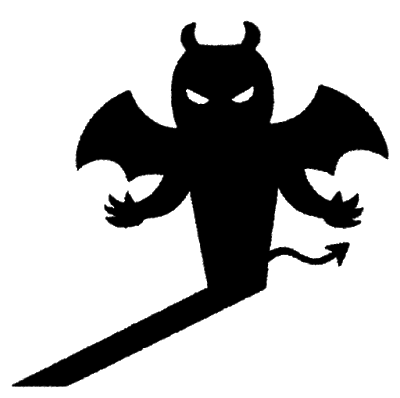
\includegraphics[width=0.95\textwidth]{img/akuma_shadow.png}
      \end{center}
    \end{column}
    \begin{column}{0.6\textwidth}
      \begin{center}
        \simplecallout{+}{blue!30}{誰が確率を計算するの?}
        \simplecallout{-}{green!30}{運営の古典コンピュータ?}
      \end{center}
    \end{column}
    \begin{column}{0.2\textwidth}
      \begin{center}
        
\includegraphics[width=0.95\textwidth]{img/question_head_gakuzen_girl.png}
      \end{center}
    \end{column}
  \end{columns}

  \begin{center}
    \simplecallout{+}{red!30}{運営の実装が正しい確率に従っているのか?}
  \end{center}
\end{frame}

\begin{frame}
  \frametitle{抽選とは?}

  \begin{columns}
    \begin{column}{0.8\textwidth}
      \begin{itemize}
        \item 「宝くじ」といった抽選では景品が1億円など高額になる
        \item ソーシャルゲームのガチャの不正疑惑により、
        運営会社の株価がストップ安になったり、
        本当に確率が実際と異っていたことがある\ce{😰}
      \end{itemize}
    \end{column}
    \begin{column}{0.2\textwidth}
      \begin{center}
        \begin{figure}[h]
          
\includegraphics[width=\textwidth]{img/toushika_kabunushi_shock.png}
        \end{figure}
      \end{center}
    \end{column}
  \end{columns}

  \pause
  \begin{center}
    \simplecallout{+}{red!30}{%
      抽選の公平性への疑惑が会社の信用に影響することもある
    }
  \end{center}

  \pause
  \begin{itemize}
    \item 抽選を公平にすることは社会的に非常に重要である
  \end{itemize}
\end{frame}

\begin{frame}
  \frametitle{公平な抽選}

  \pause
  \begin{block}{公平な抽選}
    \begin{itemize}
      \item 参加者にとっても運営にとっても、抽選による景品の出現確率が実装に基づいて明らかである
      \item 悪意を持つ参加者や、悪意を持つ運営による片方にとって有利な確率操作ができない
    \end{itemize}
  \end{block}

  \pause
  \begin{itemize}
    \item 公平な抽選の方法として古典コンピュータではたとえば次のやり方がある
    \begin{enumerate}
      \item \textbf{ブロックチェーン}を利用する方法
      \item \textbf{コミットメント}を利用する方法
    \end{enumerate}
  \end{itemize}
\end{frame}

\begin{frame}
  \frametitle{1bitの抽選 --- コイントス}

  \pause
  \begin{exampleblock}{}
    \begin{columns}
      \begin{column}{0.8\textwidth}
        \begin{enumerate}
          \item<+-> 今、``紙''と``封筒''がある
          \item<+-> アリスが紙に\textbf{表}または\textbf{裏}を書き込み
          それを封筒に入れる
          \item<+-> ボブがコイントスをする
          \item<+-> アリスとボブは封筒を開封する
          \begin{itemize}
            \item 紙に書かれた表裏とコイントスの結果が等しければ、
            アリスは景品を得る
            \item そうでなければ景品を得ない
          \end{itemize}
        \end{enumerate}
      \end{column}
      \begin{column}{0.2\textwidth}
        \begin{center}
          \uncover<2->{
            \begin{figure}[h]
              
\includegraphics[width=0.5\textwidth]{img/document_syorui_fuutou.png}
            \end{figure}
          }
          \uncover<4->{
            \begin{figure}[h]
              
\includegraphics[width=0.5\textwidth]{img/sports_coin_toss.png}
            \end{figure}
          }
        \end{center}
      \end{column}
    \end{columns}
  \end{exampleblock}

  \begin{itemize}
    \item<+-> このとき次の2つが重要となる
    \begin{enumerate}
      \item \label{enum:hiding}
      ボブは封筒の中の紙に書かれた文字を読むことができない
      \item \label{enum:binding}
      アリスは紙に書いた裏表を変更することができない
    \end{enumerate}

    \item<+-> \ballref{enum:hiding}が隠蔽、\ballref{enum:binding}が束縛となる
  \end{itemize}
\end{frame}

\begin{frame}
  \frametitle{隠蔽と束縛}

  \pause
  \begin{itemize}
    \item<+-> コイントスが公平になるためには隠蔽・束縛が完全である必要がある

    \item<+-> ところが両方を完全にすることは、
    たとえ量子コンピュータを利用したとしてもできない%
    \footnote[frame]{このことは背理法で証明できる。}
    
    \item<+-> 古典コンピュータでは片方を完全に、
    もう片方を計算の複雑さに依存させることで解決している
  \end{itemize}

  \uncover<+->{
    \begin{center}
      \simplecallout{+}{red!30}{つまり計算資源が多い方が有利!}
   
      \simplecallout{-}{cyan!30}{完全な公平ではない}
   
      \simplecallout{+}{green!30}{そこで\textbf{量子コンピュータ}を利用する}
    \end{center}
  }
\end{frame}

\section{プロジェクトの目的・成果}

\begin{frame}
  \centering
  {\Huge プロジェクトの目的・成果}
\end{frame}

\begin{frame}
  \frametitle{プロジェクトの目的・成果}

  \pause
  \begin{itemize}
    \item<+-> 量子コンピュータのシミュレーターを利用し、
    それを用いて量子コンピュータを用いる抽選システムソフトウェアの開発

    \item<+-> 開発したソフトウェアの無償公開
    \begin{itemize}
      \item \url{https://github.com/y-yu/qrand}
    \end{itemize}
    \simplecallout{+}{green!30}{%
      この後のスライドで一部を解説!
    }%

    \item<+-> 開発した抽選システムのドキュメント執筆、
    ソフトウェアの性能や課題の考察(今後の予定)
  \end{itemize}
\end{frame}

\begin{frame}
  \frametitle{量子コイントス}

  \pause
  \begin{columns}
    \begin{column}{0.7\textwidth}
      \begin{itemize}
        \item<+-> 量子コンピュータの確率的な性質を利用するコイントス
      \end{itemize}
    \end{column}
    \begin{column}{0.3\textwidth}
      \begin{figure}[h]
        \uncover<.->{
          
\includegraphics[width=0.5\textwidth]{img/sports_coin_toss.png}
        }
      \end{figure}
    \end{column}
  \end{columns}
  
  \begin{itemize}
    \item<+-> 量子コンピュータのコイントスは不正が\textbf{等しい確率}で行える
    \begin{itemize}
      \item たとえば40\%の確率で運営が不正できるならば、
      40\%の確率で参加者も不正できる
      \item 古典コンピュータではどちらか側しか不正できない
    \end{itemize}

    \item<+-> あとは何度もコイントスしていくと任意の景品に対応させられる
  \end{itemize}

  \begin{itemize}
    \item<+-> 量子コイントスはいくつかのプロトコルが提案されている\cite{Bennett2014QuantumCP, PhysRevA.80.062321}などがある
    \item<+-> このスライドでロス耐性プロトコル\cite{PhysRevA.80.062321}と
    デモ実装を紹介する
  \end{itemize}
\end{frame}

\newcommand{\天国}{\textcolor{cyan}{\ket{\text{天国}}}}
\newcommand{\地獄}{\textcolor{cyan}{\ket{\text{地獄}}}}
\newcommand{\生}{\textcolor{orange}{\ket{\text{生}}}}
\newcommand{\死}{\textcolor{orange}{\ket{\text{死}}}}

\begin{frame}
  \frametitle{実装の説明}

  \pause
  \begin{itemize}
    \item<+-> 量子シミュレーターとしてQulacs\cite{qulacs}を利用
    \item<+-> Webサーバー・JSON通信部分はPythonとFlaskを利用
  \end{itemize}

  \uncover<.->{
    \begin{figure}[h]
      \footnotesize
      \begin{tikzpicture}[scale=1, block/.style = {rectangle, draw=black, thick, text width=4em, align=center, rounded corners, minimum height=2em}, tx/.style = {rectangle, draw=black, very thick, text width=2em, align=center, minimum height=1em}]
        \draw (0, 0) node[block] (A) {Webフロント};
        \draw (3, 0) node[block] (B) {クライアント};
        \draw (6, 0) node[block] (C) {サーバー};
                
        \draw (1.4, 0.3) node (xhr) {XHR};
        \draw (4.4, 0.3) node (json) {JSON};
         
        \draw[<->, very thick] (A) -- (B);
        \draw[<->, very thick] (B) -- (C);
      \end{tikzpicture}
    \end{figure}
  }

  \begin{itemize}
    \item<+-> JSONの部分が実際には量子通信となる
    
    \item<+-> 今回はエミュレーターなので、
    1量子ビットを表現する2つの複素数をJSON形式でやりとりする

    \item<+-> やりとりするのは次のような4パターンの量子ビット
    \begin{align*}
      \天国 &\equiv \sqrt{0.9}\ket{0} + \sqrt{0.1}\ket{1} ,\;
      \地獄 &\equiv \sqrt{0.1}\ket{0} - \sqrt{0.9}\ket{1} \\
      \生 &\equiv \sqrt{0.9}\ket{0} - \sqrt{0.1}\ket{1} ,\;
      \死 &\equiv \sqrt{0.1}\ket{0} + \sqrt{0.9}\ket{1}
    \end{align*}
  \end{itemize}
\end{frame}

\begin{frame}
  \frametitle{プロトコル}
  
  \begin{figure}[h]
    \footnotesize
    \begin{tikzpicture}[scale=1.3, block/.style = {rectangle, draw=black, thick, text width=7em, align=center, rounded corners, minimum height=2em}, tx/.style = {rectangle, draw=black, very thick, text width=2em, align=center, minimum height=1em}]
      \draw (-2, 0) node[block] (B) {クライアント(参加者)};
      \draw (1.5, 0.3) node {
        \scriptsize
        \begin{tabular}{|c|c|c|}
          \hline
          \diagbox{$a$}{$x$} & $0$       & $1$    \\ \hline
          $0$                & $\天国$    & $\地獄$ \\ \hline
          $1$                & $\生$      & $\死$  \\ \hline
        \end{tabular}
      };
      \draw (5, 0) node[block] (C) {サーバー(運営)};
      \draw[->, very thick] (-2.5,-0.5) -- (5.8,-0.5);
      \draw[align=left] (0.8, -0.8) node (p1) {%
        \ballcircle{1}それぞれ1ビットの$a,x$を用いて4つから \\
        1量子ビットを選びサーバーへ送る
      };
      \draw[<-, very thick] (-2.5,-1.2) -- (5.8,-1.2);
      \draw[align=left] (4.3, -2) node (p2) {%
        \ballcircle{2}1ビット乱数$\hat{a},b$を生成し \\
        $\hat{a} = 0$なら$\{\天国, \地獄 \}$で \\
        $\hat{a} = 1$なら$\{\生, \死 \}$で測定し\\
        結果を$\hat{x}$として保存し$b$を送信
      };
      \draw[->, very thick] (-2.5, -3) -- (5.8, -3);
      \draw[align=left] (-1.5, -3.2) node (p3) {%
        \ballcircle{3}$a,x$を公開
      };
      \draw[align=left] (4.3, -3.8) node (p4) {%
        \ballcircle{4}$a = \hat{a}$ならば$x = \hat{x}$を検証
      };
      \draw[<-, very thick] (-2.5, -4.2) -- (5.8, -4.2);
      \draw[align=left] (4.5, -4.5) node (p5) {%
        \ballcircle{5}$x \, \mathtt{XOR}\, b$を結果とする
      };
    \end{tikzpicture}
  \end{figure}
\end{frame}

\begin{frame}
  \frametitle{公平性の説明}

  \pause
  \begin{itemize}
    \item<+-> 参加者は送信する量子ビットを次の中から選択する
  \end{itemize}

  \begin{columns}
    \begin{column}{0.5\textwidth}
      \begin{table}[h]
        \footnotesize
        \begin{tabular}{|c|c|c|}
          \hline
          \diagbox{$a$}{$x$} & $0$       & $1$    \\ \hline
          $0$                & $\天国$    & $\地獄$ \\ \hline
          $1$                & $\生$      & $\死$  \\ \hline
        \end{tabular}
      \end{table}
    \end{column}
    \begin{column}{0.5\textwidth}
      \begin{figure}[h]
        \footnotesize
        \begin{blochsphere}[radius=0.15\textwidth, tilt=15,rotation=-20,opacity=0]
          \drawBallGrid[style={opacity=0.2}]{40}{40}
       
          \drawAxis[style={cyan}]{0}{0};
          \drawAxis[style={orange}]{90}{0};
           
          \labelLatLon{up}{72}{0};
          \labelLatLon{down}{-108}{90};
          \labelLatLon{left}{0}{0};
          \labelLatLon{right}{180}{0};
          \node[above] at (up) {$\天国$};
          \node[below] at (down) {$\地獄$};
          \node[above] at (left) {$\生$};
          \node[above] at (right) {$\死$};
        \end{blochsphere}
      \end{figure}
    \end{column}
  \end{columns}

  \begin{columns}
    \begin{column}{0.1\textwidth}
      \uncover<4->{
        
\includegraphics[width=\textwidth]{img/cat_russian_blue.png}
      }
    \end{column}
    \begin{column}{0.9\textwidth}
      \begin{itemize}
        \item<+-> 図のように$a$が同じ(= 色が同じ)なら直交する
       
        \item<+-> たとえば量子ビット$\地獄$の測定を考える
        \begin{description}
          \begin{columns}
            \begin{column}{0.4\textwidth}            
              \item[$\{\天国, \地獄\}$で測定した場合]\mbox{}\\
              常に$\地獄$が出力
            \end{column}
            \begin{column}{0.45\textwidth}           
               \item[$\{\生, \死\}$で測定した場合]\mbox{}\\
               $\生, \死$のいずれかが確率で出力
            \end{column}
          \end{columns}
        \end{description}
      \end{itemize}
    \end{column}
  \end{columns}
\end{frame}

\begin{frame}
  \frametitle{公平性の説明}

  \begin{columns}
    \begin{column}{0.2\textwidth}
      \begin{figure}[h]
        \footnotesize
        \begin{blochsphere}[radius=0.50\textwidth, tilt=15,rotation=-20,opacity=0]
          \drawBallGrid[style={opacity=0.2}]{40}{40}
       
          \drawAxis[style={cyan}]{0}{0};
          \drawAxis[style={orange}]{90}{0};
           
          \labelLatLon{up}{90}{0};
          \labelLatLon{down}{-90}{90};
          \labelLatLon{left}{0}{0};
          \labelLatLon{right}{180}{0};
          \node[above] at (up) {$\天国$};
          \node[below] at (down) {$\地獄$};
          \node[above] at (left) {$\生$};
          \node[above] at (right) {$\死$};
        \end{blochsphere}
      \end{figure}
    \end{column}
    \begin{column}{0.8\textwidth}
      \begin{itemize}
        \item<+-> たとえば参加者が$\地獄(a = 0)$を選んだとして、
        運営は$\{\天国, \地獄\}$か$\{\生, \死\}$のいずれで測定するか決める
        \begin{enumerate}
          \item 運営が$\{\天国, \地獄\}$を選べば\textbf{検証ができる}
          \item 一方で$\{\生, \死\}$を選べば\textbf{検証ができない}
        \end{enumerate}

        \item<+-> つまり、運営は測定結果$\hat{x}$を得るが、これは
        コミットメントとなるのかランダムな出力なのか
        参加者の$a$を知るまで分からない
      \end{itemize}
    \end{column}
  \end{columns}

  \begin{itemize}
    \item<+-> 参加者がこの後、どの量子ビットを利用したか公開するとき
    運営の得た測定結果$\hat{x}$を知らないため、
    コミットメントされているのかどうかが分からない
    \begin{itemize}
      \item つまり確率でズルできる\ce{😈}が、確率で失敗する
    \end{itemize}

    \item<+-> このように量子コイントスでは古典のコミットメントのように
    計算量でどちらかが有利になるということはない
  \end{itemize}
\end{frame}


\begin{frame}
  \centering
  {\Huge デモ動画}

  \begin{itemize}
    \item ここまで紹介したプロトコルを実際に試して、
    またチート(不正)してみることもできる機能のデモ
    
    \item \url{https://github.com/y-yu/qrand}%
  \end{itemize}
\end{frame}

\section{まとめ}

\begin{frame}
  \frametitle{まとめ}

  \pause
  \begin{itemize}
    \item<+-> なんらかの計算速度を向上させるという利用用途以外にも
    量子コンピュータにはこのような抽選への利用など様々な応用がある

    \item<+-> 今回の発表では時間の関係で割愛したが、
    参加者・運営が互いにチートする場合や、
    あえて運営が途中まで勝たせる戦略などがあり、それは近々文書にまとめて
    公開したい

    \item<+-> 運営 \textit{vs} 参加者の抽選は公平に不正ができたとしても
    本当に公平であるのかについて引き続き考えたい
    \begin{itemize}
      \item 抽選の景品に完全な順序がつく(たとえばお金)なら簡単だが、
      ゲームの景品などは必ずしも順序がつくとは限らない
      
      \item したがって運営は参加者にとってコインの「裏か表のどちらが有利か?」ということ
      知らないことがある?
    \end{itemize}
    
    \item<+-> 今回の実装は量子通信回線を前提としているのが実用化への課題である。
    また抽選の多人数化などについても今後検討したい
  \end{itemize}
\end{frame}

\section*{参考文献}

\begin{frame}[allowframebreaks]
  \frametitle{参考文献}

  \bibliographystyle{junsrt_url}
  \bibliography{ref}
\end{frame}

\begin{frame}
  \centering
  {\Huge Thank you for your attention!}
\end{frame}

\appendix

\begin{frame}
  \frametitle{質疑用のスライド}

  \tableofcontents
\end{frame}

\section{古典コンピュータによる実装}

\subsection{ブロックチェーン}
 
\begin{frame}
  \frametitle{ブロックチェーン}
 
  \begin{block}{ブロックチェーン}
    \begin{columns}
      \begin{column}{0.8\textwidth}
        \begin{itemize}
          \item マスターが複数あるデータベース
          
          \item ブロックチェーンを管理する者(マイナー)は
          時間のかかるハッシュ計算をし報酬を得る
          \begin{itemize}
            \item マイナーは1つ前のブロックのハッシュ値と
            マイナーが作成した乱数をハッシュ関数へ投入し、
            先頭$n$ビットが$0$な場合に報酬を得る
          \end{itemize}
        \end{itemize}
      \end{column}
      \begin{column}{0.2\textwidth}
        \begin{center}
          \begin{figure}[h]
            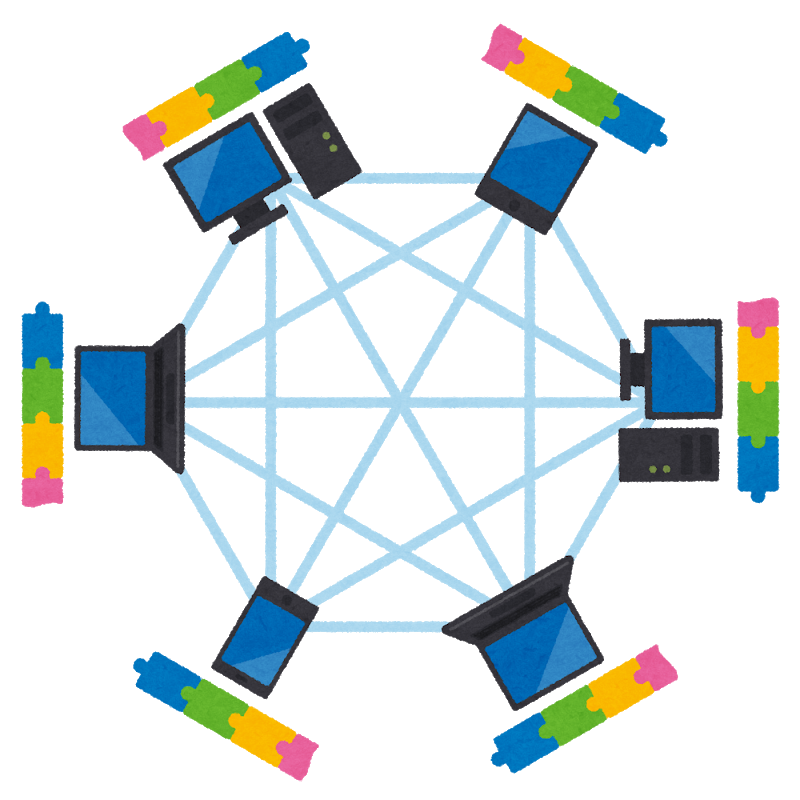
\includegraphics[width=0.8\textwidth]{img/network_blockchain.png}
          \end{figure}
        \end{center}
      \end{column}
    \end{columns}
  \end{block}
  
  \begin{itemize}
    \item マイナーが計算する先頭$n$ビットが$0$なハッシュ値は
    残りのビットが予測困難なため、それを公平な抽選へ利用する
  \end{itemize}
\end{frame}
 
\begin{frame}
  \frametitle{ブロックチェーン}
 
  \begin{itemize}
    \item ブロックチェーンを利用した公平な抽選は
    マイナーが公平なことに依存する
    \begin{itemize}
      \item マイナーが計算したハッシュ値による抽選の結果が
      マイナーにとって不都合な場合、ブロックチェーンの報酬を放棄することで有利になる
    \end{itemize}
 
    \item マイナーは合理的な存在であると考えられるから
    抽選の景品の価値がブロックチェーンの報酬を越える場合、
    マイナーは抽選の景品を優先する
  \end{itemize}
 
  \begin{center}
    \begin{tikzpicture}
      \calloutquote[width=11.5cm,position={(0.9,-0.2)},fill=red!30,rounded corners]{景品の価値がいくらのとき、マイナーは景品を優先するのか?}
    \end{tikzpicture}
  \end{center}
 
  \begin{itemize}
    \item 記事によると、
    景品の価値が\textbf{約150万円}以上のとき%
    \footnote[frame]{この計算の当時とは為替が違うため、現在はもう少々必要である}
 
    \item 1億円など高額が動く抽選へ利用した場合に完璧とは言えない
  \end{itemize}
\end{frame}
 
\subsection{コミットメント}

\begin{frame}
  \frametitle{コミットメント}

  \begin{itemize}
    \item 公平なコイントスは次のようなゲームを例に説明できる
  \end{itemize}

  \begin{exampleblock}{}
    \begin{columns}
      \begin{column}{0.8\textwidth}
        \begin{enumerate}
          \item 今、``紙''と``封筒''がある
          \item アリスが紙に\textbf{表}または\textbf{裏}を書き込み
          それを封筒に入れる
          \item ボブがコイントスをする
          \item アリスとボブは封筒を開封する
          \begin{itemize}
            \item 紙に書かれた表裏とコイントスの結果が等しければ、
            アリスは景品を得る
            \item そうでなければ景品を得ない
          \end{itemize}
        \end{enumerate}
      \end{column}
      \begin{column}{0.2\textwidth}
        \begin{center}
          \begin{figure}[h]
            
\includegraphics[width=0.5\textwidth]{img/document_syorui_fuutou.png}
          \end{figure}
          \begin{figure}[h]
            
\includegraphics[width=0.5\textwidth]{img/sports_coin_toss.png}
          \end{figure}
        \end{center}
      \end{column}
    \end{columns}
  \end{exampleblock}

  \begin{itemize}
    \item このとき次の2つが重要となる
    \begin{enumerate}
      \item \label{enum:hiding}
      ボブは封筒の中の紙に書かれた文字を読むことができない
      \item \label{enum:binding}
      アリスは紙に書いた裏表を変更することができない
    \end{enumerate}

    \item \ballref{enum:hiding}が隠蔽、\ballref{enum:binding}が束縛となる
  \end{itemize}
\end{frame}

\begin{frame}
  \frametitle{コミットメント}

  \begin{itemize}
    \item コイントスが公平になるためには隠蔽・束縛が完全である必要がある

    \item ところが両方を完全にすることは、
    たとえ量子コンピュータを利用したとしてもできない
    \begin{itemize}
      \item 古典コンピュータでは片方を完全に、
      もう片方を計算の複雑さに依存させることで解決している
    \end{itemize}
  \end{itemize}

  \begin{center}
    \begin{tikzpicture}
      \calloutquote[width=7cm,position={(0.9,-0.2)},fill=red!30,rounded corners]{つまり計算資源が多い方が有利!}
    \end{tikzpicture}
  \end{center}

  \begin{itemize}
    \item これは完全な公平ではない
  \end{itemize}

  \begin{center}
    \begin{tikzpicture}
      \calloutquote[width=7cm,position={(-0.5,-0.2)},fill=green!30,rounded corners]{そこで\textbf{量子コンピュータ}を利用する}
    \end{tikzpicture}
  \end{center}
\end{frame}

\section{アリス・ボブの不正}

\begin{frame}
  \frametitle{アリス・ボブの不正}

  \begin{itemize}
    \item プロトコルを意図的に無視すれば不正することができる
    \begin{itemize}
      \item これは確率で不正をしようとしたことがバレてしまう
    \end{itemize}

    \item アリスの最適な不正もボブの最適な不正も同じ割合で成功し
    同じ割合で失敗する
  \end{itemize}

  \uncover<+->{
    \simplecallout{-}{cyan!20}{%
      どうしてそうなるの?
    }
  }

  \uncover<+->{
    \simplecallout{+}{green!20}{%
      そうなるように$\sqrt{0.9}$とか$\sqrt{0.1}$を選んだから!
    }
  }
\end{frame}

\end{document}
